\documentclass[10pt]{article}
\usepackage[a4paper,margin=13mm]{geometry}
\usepackage[T1]{fontenc}
\usepackage{lmodern}
\usepackage{microtype}
\usepackage{amsmath,amssymb}
\usepackage{booktabs,tabularx,array,multirow}
\usepackage[dvipsnames,table]{xcolor}
\usepackage{tikz}
\usetikzlibrary{arrows.meta,positioning,fit,backgrounds,calc,shapes.geometric,matrix}
\usepackage[colorlinks=true,linkcolor=MidnightBlue,urlcolor=MidnightBlue]{hyperref}
\usepackage{enumitem}
\setlist{nosep,leftmargin=*}
\pagestyle{plain}
\setlength{\parindent}{0pt}
\setlength{\parskip}{4pt}
\renewcommand{\arraystretch}{1.16}

\definecolor{shared}{HTML}{2E7D32}
\definecolor{partial}{HTML}{E58E26}
\definecolor{paperonly}{HTML}{8E44AD}
\definecolor{legoOnly}{HTML}{2471A3}
\definecolor{palegreen}{HTML}{EAF6EA}
\definecolor{paleorange}{HTML}{FFF2DF}
\definecolor{palepurple}{HTML}{F1EAF7}
\definecolor{paleblue}{HTML}{E8F2FA}
\definecolor{ink}{HTML}{25313C}

\tikzset{
  box/.style={draw=ink!55,rounded corners=2pt,text width=42mm,align=center,inner sep=4pt,font=\small,fill=white},
  sharedbox/.style={box,draw=shared,fill=palegreen,line width=.8pt},
  partialbox/.style={box,draw=partial,fill=paleorange,line width=.8pt},
  paperbox/.style={box,draw=paperonly,fill=palepurple,line width=.8pt},
  legobox/.style={box,draw=legoOnly,fill=paleblue,line width=.8pt},
  arr/.style={-{Stealth[length=2.2mm]},line width=.65pt,draw=ink!75},
  dasharr/.style={arr,dashed},
  title/.style={font=\bfseries\large,text=ink},
  tinylabel/.style={font=\scriptsize,text=ink!70,text width=18mm,align=center}
}

\newcommand{\file}[1]{\texttt{\detokenize{#1}}}
\newcommand{\yes}{\textcolor{shared}{\bfseries common}}
\newcommand{\partly}{\textcolor{partial}{\bfseries partial}}
\newcommand{\no}{\textcolor{paperonly}{\bfseries additional}}

\begin{document}

% ---------------------------------------------------------------------------
\begin{center}
{\fontsize{23}{27}\selectfont\bfseries The Dobbertin LEGO Atlas}\par
\vspace{2mm}
{\large Building blocks shared by two papers and their Lean formalizations}\par
\vspace{3mm}
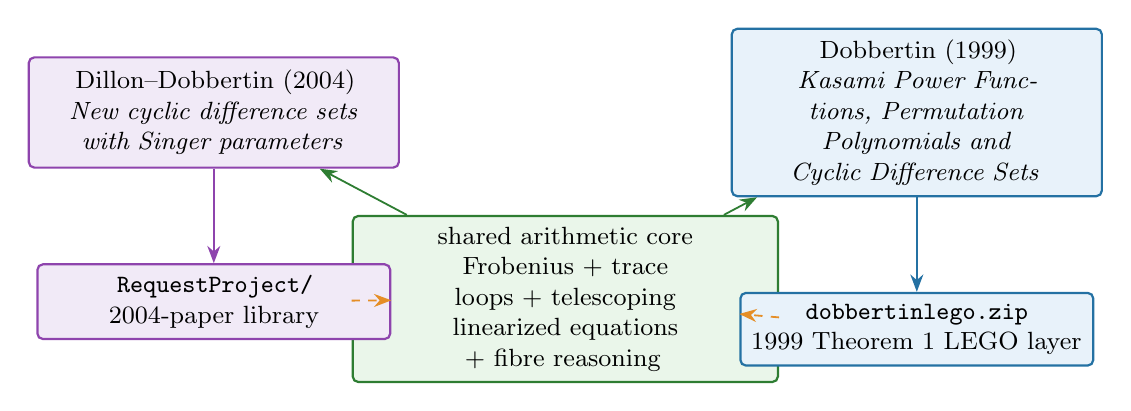
\begin{tikzpicture}[node distance=7mm and 14mm]
  \node[paperbox,minimum width=47mm,minimum height=14mm] (p04) {Dillon--Dobbertin (2004)\\\emph{New cyclic difference sets\\with Singer parameters}};
  \node[legobox,minimum width=47mm,minimum height=14mm,right=42mm of p04] (p99) {Dobbertin (1999)\\\emph{Kasami Power Functions, Permutation\\Polynomials and Cyclic Difference Sets}};
  \node[sharedbox,minimum width=54mm,below=13mm of $(p04)!0.5!(p99)$] (core) {shared arithmetic core\\Frobenius $+$ trace loops $+$ telescoping\\linearized equations $+$ fibre reasoning};
  \node[paperbox,below=12mm of p04] (lib) {\file{RequestProject/}\\2004-paper library};
  \node[legobox,below=12mm of p99] (zip) {\file{dobbertinlego.zip}\\1999 Theorem 1 LEGO layer};
  \draw[arr,shared] (core)--(p04); \draw[arr,shared] (core)--(p99);
  \draw[arr,paperonly] (p04)--(lib); \draw[arr,legoOnly] (p99)--(zip);
  \draw[dasharr,partial] (core)--(lib); \draw[dasharr,partial] (core)--(zip);
\end{tikzpicture}
\end{center}

\vspace{2mm}
\colorbox{paleorange}{\parbox{0.96\linewidth}{
\textbf{Short answer.} The projects share a real and reusable lower layer, but they are \emph{not} the same construction.  The ZIP is centered on Theorem~1 of a 1999 Dobbertin paper; the uploaded paper and the \file{RequestProject} library follow the much broader 2004 Dillon--Dobbertin paper.  Frobenius, trace/partial-trace loops, telescoping, linearized polynomials, and fibre uniqueness can be built from essentially the same bricks.  Hadamard analysis, Singer difference sets, Dickson tori, MCM--Dickson identities, characteristic-two quadratic forms, cubic characters/Gauss sums, and design inequivalence require further brick families already represented in \file{RequestProject/Foundations}.}}

\vfill
\begin{center}\small
Colour code: \textcolor{shared}{\rule{8mm}{2mm} shared} \quad
\textcolor{partial}{\rule{8mm}{2mm} adaptable/partial} \quad
\textcolor{paperonly}{\rule{8mm}{2mm} 2004-specific families} \quad
\textcolor{legoOnly}{\rule{8mm}{2mm} 1999-LEGO presentation}.\\
Page references below use the printed journal pagination; the parenthesized number is the page in the supplied 48-page PDF.
\end{center}
\newpage

% ---------------------------------------------------------------------------
\section*{1. First separate the two source papers}

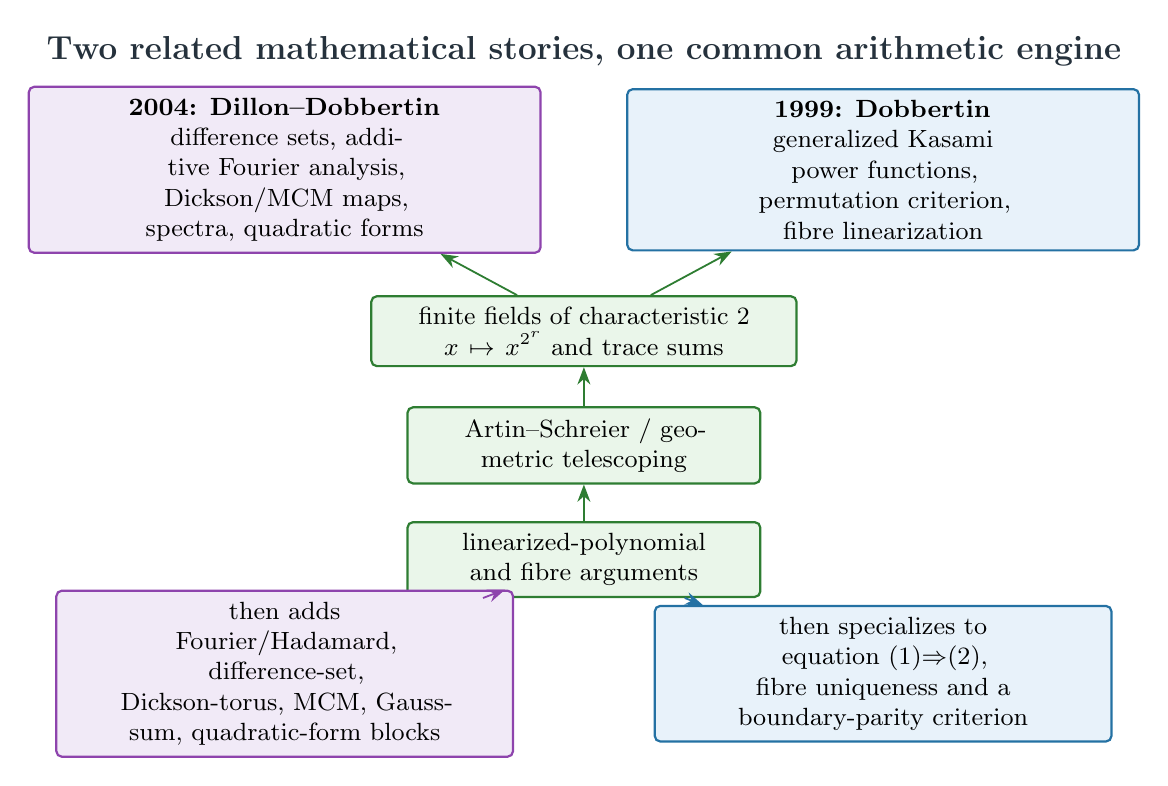
\begin{tikzpicture}[node distance=8mm and 9mm]
\node[title] at (7.5,2.0) {Two related mathematical stories, one common arithmetic engine};
\node[paperbox,minimum width=65mm,minimum height=17mm] (A) at (3.7,.5)
 {\textbf{2004: Dillon--Dobbertin}\\difference sets, additive Fourier analysis,\\Dickson/MCM maps, spectra, quadratic forms};
\node[legobox,minimum width=65mm,minimum height=17mm] (B) at (11.3,.5)
 {\textbf{1999: Dobbertin}\\generalized Kasami power functions,\\permutation criterion, fibre linearization};
\node[sharedbox,minimum width=54mm] (F) at (7.5,-1.55)
 {finite fields of characteristic $2$\\$x\mapsto x^{2^r}$ and trace sums};
\node[sharedbox] (T) at (7.5,-3.0) {Artin--Schreier / geometric telescoping};
\node[sharedbox] (L) at (7.5,-4.45) {linearized-polynomial and fibre arguments};
\draw[arr,shared] (F)--(A); \draw[arr,shared] (F)--(B);
\draw[arr,shared] (T)--(F); \draw[arr,shared] (L)--(T);
\node[paperbox,minimum width=58mm] (PA) at (3.7,-5.9)
 {then adds Fourier/Hadamard, difference-set,\\Dickson-torus, MCM, Gauss-sum, quadratic-form blocks};
\node[legobox,minimum width=58mm] (PB) at (11.3,-5.9)
 {then specializes to equation (1)$\Rightarrow$(2),\\fibre uniqueness and a boundary-parity criterion};
\draw[arr,paperonly] (L)--(PA); \draw[arr,legoOnly] (L)--(PB);
\end{tikzpicture}

\subsection*{What the ZIP actually contains}
The archive's top-level documentation explicitly names the 1999 paper and describes the path
\[
 \text{Frobenius}\to\text{Loop}\to\text{Assembly}\to
 \text{FiberReduction}\to\text{FiberUniqueness}\to\text{Theorem 1}.
\]
Its self-contained generic core is concentrated in \file{Endo.lean}, \file{Frobenius.lean},
\file{Loop.lean}, and \file{Assembly.lean}; it also supplies algebraic, categorical, object-first,
and Mac Lane presentations of that core.

\textbf{Packaging caveat.}  The archive is not, by itself, the complete 1999 formalization:
\file{FiberReduction.lean}, \file{FiberUniqueness.lean}, and \file{Theorem1.lean} import
\file{Dobbertin.Theorem1.*} modules that are not present in the ZIP.  Thus the generic LEGO
core is reusable, while the end-to-end facade expects another library to be available.

\subsection*{What the current project contains}
\file{RequestProject/} is a modular transcription and growing proof library for the 2004 paper.
Its paper-facing files mirror Sections 1--8 and Appendix A; its \file{Foundations/} directory
contains the bottom-up reusable infrastructure.  Some declarations remain explicit \file{sorry}
boxes, so the atlas distinguishes \emph{available bricks and interfaces} from a fully completed proof.
\newpage

% ---------------------------------------------------------------------------
\section*{2. The common LEGO spine}

\begin{center}
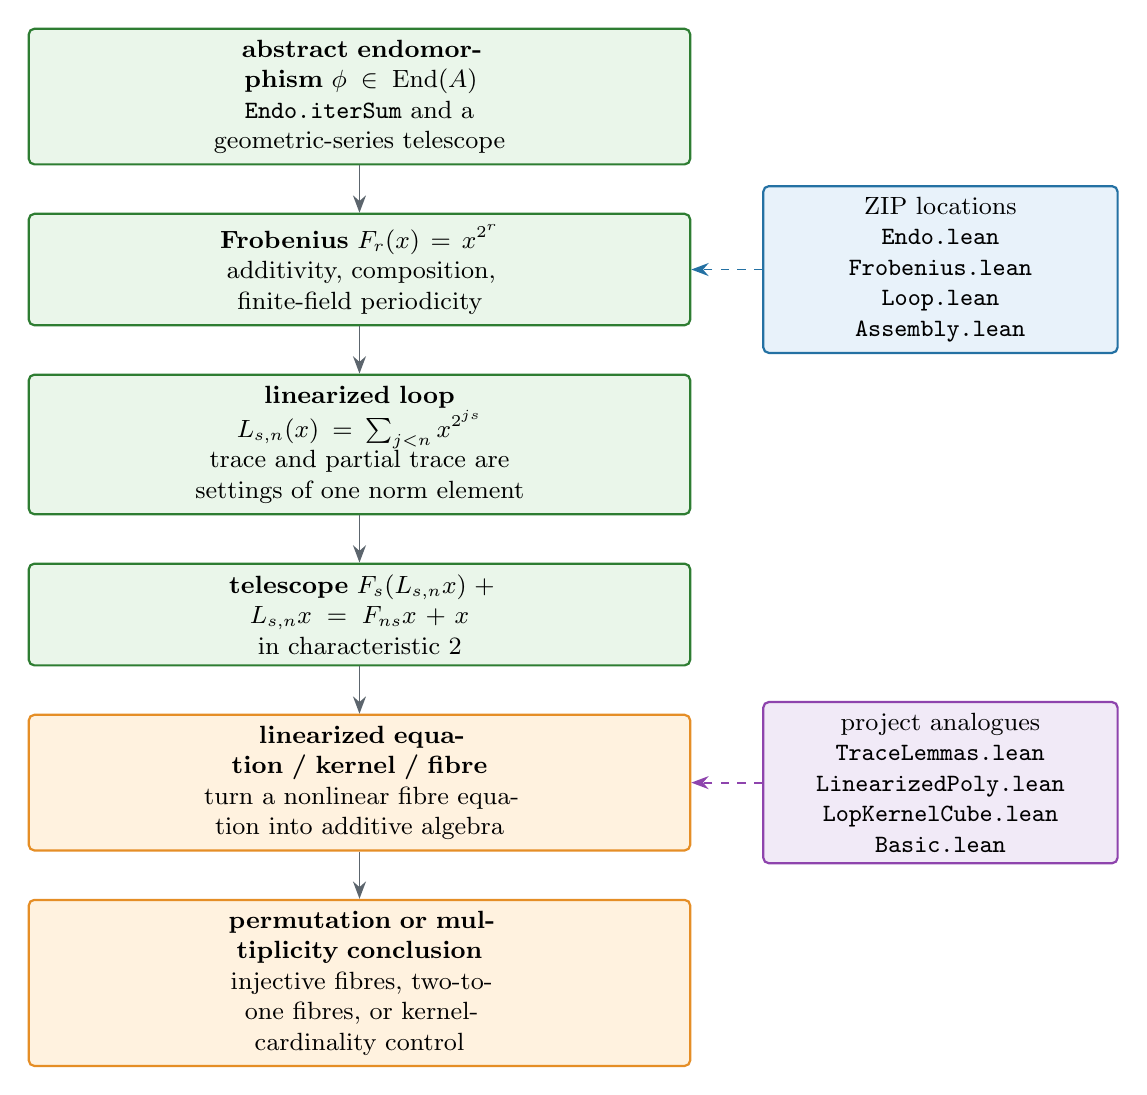
\begin{tikzpicture}[node distance=6mm]
\node[sharedbox,minimum width=84mm] (e) {\textbf{abstract endomorphism} $\phi\in\operatorname{End}(A)$\\\file{Endo.iterSum} and a geometric-series telescope};
\node[sharedbox,minimum width=84mm,below=of e] (f) {\textbf{Frobenius} $F_r(x)=x^{2^r}$\\additivity, composition, finite-field periodicity};
\node[sharedbox,minimum width=84mm,below=of f] (l) {\textbf{linearized loop} $L_{s,n}(x)=\sum_{j<n}x^{2^{js}}$\\trace and partial trace are settings of one norm element};
\node[sharedbox,minimum width=84mm,below=of l] (t) {\textbf{telescope} $F_s(L_{s,n}x)+L_{s,n}x=F_{ns}x+x$ in characteristic $2$};
\node[partialbox,minimum width=84mm,below=of t] (q) {\textbf{linearized equation / kernel / fibre}\\turn a nonlinear fibre equation into additive algebra};
\node[partialbox,minimum width=84mm,below=of q] (p) {\textbf{permutation or multiplicity conclusion}\\injective fibres, two-to-one fibres, or kernel-cardinality control};
\foreach \x/\y in {e/f,f/l,l/t,t/q,q/p}\draw[arr] (\x)--(\y);
\node[legobox,right=9mm of f,minimum width=45mm] (z1) {ZIP locations\\\file{Endo.lean}\\\file{Frobenius.lean}\\\file{Loop.lean}\\\file{Assembly.lean}};
\node[paperbox,right=9mm of q,minimum width=45mm] (z2) {project analogues\\\file{TraceLemmas.lean}\\\file{LinearizedPoly.lean}\\\file{LopKernelCube.lean}\\\file{Basic.lean}};
\draw[dasharr,legoOnly] (z1)--(f); \draw[dasharr,paperonly] (z2)--(q);
\end{tikzpicture}
\end{center}

\begin{tabularx}{\linewidth}{>{\bfseries}p{25mm} X X}
\toprule
Brick & \file{dobbertinlego.zip} & 2004 formalization / mathematical use \\
\midrule
Endomorphism norm & \file{iterSum}, \file{iterSum_telescope}, \file{normElt} & General pattern behind trace loops; reusable in \file{LinearizedPoly} and trace identities.\\
Frobenius & \file{frob}, \file{frobEndo}, periodicity & Field powers and trace invariance throughout; explicit support in \file{TraceLemmas}.\\
Trace loop & \file{loop}, \file{trace}, \file{partialTrace}, \file{numeratorSum} & Absolute/relative traces in Sections 1, 4, 7, 8 and Appendix A.\\
Linearization & equation (1)$\Rightarrow$ affine Frobenius equation (2) & MCM telescoping, $L_{k,a}$ kernels, quadratic-form radicals.\\
Fibres & uniqueness and boundary collisions & multiplicity functions, 2-to-1 maps, Dickson fibres, kernel-size arguments.\\
\bottomrule
\end{tabularx}

\textbf{The correct reuse claim is structural, not literal.}  The same abstract telescope can
power both developments.  The concrete equations, target maps, and final theorems differ, so an
adapter layer is needed rather than a wholesale import-and-finish operation.
\newpage

% ---------------------------------------------------------------------------
\section*{3. Where the blocks occur in the 2004 paper}

\begin{center}
\textbf{Paper route: printed pages 342--389 (PDF pages 1--48)}

\begin{tikzpicture}[node distance=5mm and 4mm]
\node[sharedbox,text width=22mm] (s1) {\S1\\trace, Frobenius, Hadamard\\342--349};
\node[paperbox,text width=18mm,right=of s1] (s2) {\S2\\known families\\349--352};
\node[partialbox,text width=24mm,right=of s2] (s3) {\S3\\Dickson fibres, MCM\\352--360};
\node[partialbox,text width=22mm,right=of s3] (s4) {\S4\\Theorem A\\361--369};
\node[paperbox,text width=20mm,right=of s4] (s56) {\S5--6\\special cases, Thm.~B\\369--371};
\node[paperbox,text width=20mm,right=of s56] (s7) {\S7\\bent spectra\\371--376};
\node[paperbox,text width=22mm,below=of s7] (s8) {\S8\\No--Chung--Yun\\376--381};
\node[paperbox,text width=28mm,left=of s8] (app) {Appendix A\\quadratic forms, Gauss sums\\381--388};
\foreach \a/\b in {s1/s2,s2/s3,s3/s4,s4/s56,s56/s7,s7/s8,s8/app}\draw[arr] (\a)--(\b);
\end{tikzpicture}
\end{center}

\begin{tabularx}{\linewidth}{p{17mm}p{23mm}X X}
\toprule
Paper place & PDF page(s) & Mathematical blocks visible there & Main Lean destination \\
\midrule
\S1, pp.~342--349 & 1--8 & $L=\mathrm{GF}(2^m)$, trace character, normalized Hadamard transform, convolution, Parseval, Singer difference-set criteria & \file{Basic}, \file{DifferenceSets}, \file{AdditiveChar}\\
\S3, pp.~352--360 & 11--19 & Dickson polynomial identity and permutation criterion (Thm.~3); fibre sizes (Prop.~5); multiplicity (Prop.~6, Thm.~7); MCM maps (Thms.~8--10) & \file{Dickson}, \file{MCM}, \file{DicksonTorus}, \file{CyclicFibre}, \file{LinearizedPoly}\\
\S4, pp.~361--369 & 20--28 & Theorem A; Lemmas A1/A2; trace substitutions and Fourier/Hadamard equivalence & \file{MainTheoremA}, \file{GaussSumTheory}, \file{QuadFormChar2}\\
\S5--6, pp.~369--371 & 28--30 & special cases; MCM--Dickson transform dictionary (Theorem B) & \file{SpecialCases}, \file{MCMDicksonRelation}\\
\S7, pp.~371--376 & 30--35 & bent functions and three-valued spectra (Thm.~11, Cor.~12) & \file{HadamardSpectrum}, \file{QuadFormChar2}\\
\S8, pp.~376--381 & 35--40 & No--Chung--Yun difference set (Thms.~13, 15 and corollaries) & \file{NoChungYun}, \file{DesignTheory}\\
App.~A, pp.~381--388 & 40--47 & rank/radical, canonical forms, Fourier spectrum of quadratic forms, trace forms, cubic Gauss sum & \file{QuadraticForms}, \file{QuadFormClassification}, \file{GaussSums}, \file{CubicCharacter}\\
\bottomrule
\end{tabularx}
\newpage

% ---------------------------------------------------------------------------
\section*{4. The 2004 formalization as a LEGO city}

\begin{center}
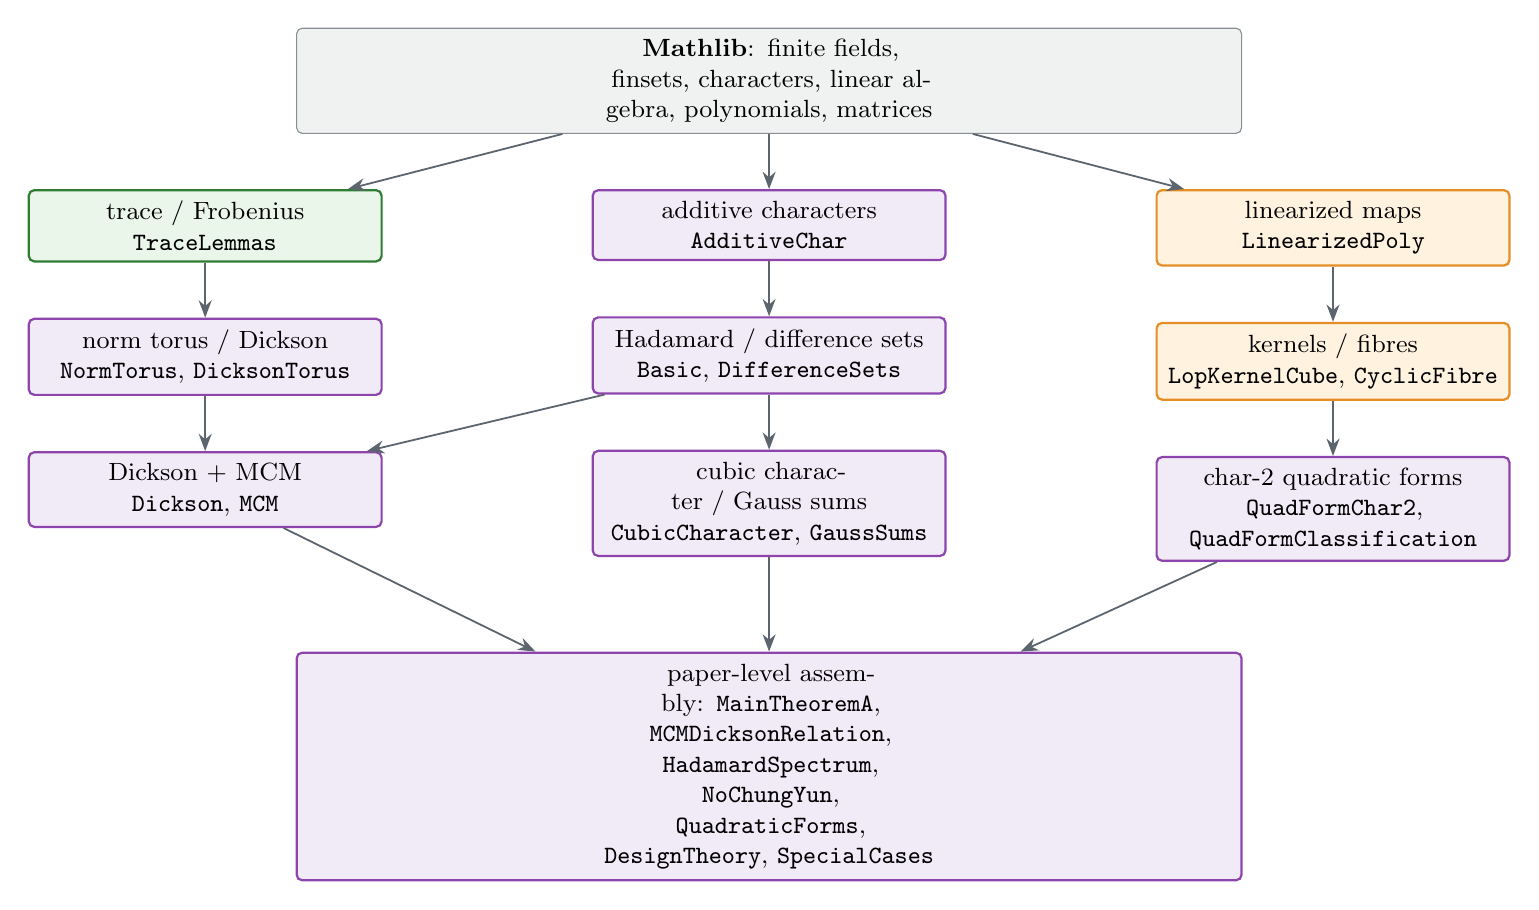
\begin{tikzpicture}[node distance=7mm and 7mm]
\node[box,fill=ink!7,minimum width=120mm] (mathlib) {\textbf{Mathlib}: finite fields, finsets, characters, linear algebra, polynomials, matrices};
\node[sharedbox,below left=of mathlib,xshift=18mm] (trace) {trace / Frobenius\\\file{TraceLemmas}};
\node[paperbox,below=of mathlib] (fourier) {additive characters\\\file{AdditiveChar}};
\node[partialbox,below right=of mathlib,xshift=-18mm] (lin) {linearized maps\\\file{LinearizedPoly}};
\node[paperbox,below=of trace] (torus) {norm torus / Dickson\\\file{NormTorus}, \file{DicksonTorus}};
\node[paperbox,below=of fourier] (had) {Hadamard / difference sets\\\file{Basic}, \file{DifferenceSets}};
\node[partialbox,below=of lin] (fib) {kernels / fibres\\\file{LopKernelCube}, \file{CyclicFibre}};
\node[paperbox,below=of torus] (dick) {Dickson + MCM\\\file{Dickson}, \file{MCM}};
\node[paperbox,below=of had] (gauss) {cubic character / Gauss sums\\\file{CubicCharacter}, \file{GaussSums}};
\node[paperbox,below=of fib] (quad) {char-$2$ quadratic forms\\\file{QuadFormChar2}, \file{QuadFormClassification}};
\node[paperbox,below=12mm of gauss,minimum width=120mm] (top) {paper-level assembly: \file{MainTheoremA}, \file{MCMDicksonRelation}, \file{HadamardSpectrum},\\\file{NoChungYun}, \file{QuadraticForms}, \file{DesignTheory}, \file{SpecialCases}};
\foreach \a/\b in {mathlib/trace,mathlib/fourier,mathlib/lin,trace/torus,fourier/had,lin/fib,torus/dick,had/dick,had/gauss,fib/quad,dick/top,gauss/top,quad/top}\draw[arr] (\a)--(\b);
\end{tikzpicture}
\end{center}

\textbf{Reading the colours.}  The green and orange columns are the best candidates for direct
conceptual reuse from the ZIP.  Purple nodes are not dispensable decoration: they encode the
extra mathematics by which the 2004 paper turns finite-field maps into cyclic difference sets,
Fourier spectra, and inequivalence results.

\begin{tabularx}{\linewidth}{>{\bfseries}p{31mm} X X}
\toprule
Family & Input supplied by the common spine & New connector required in the 2004 library \\
\midrule
Trace/Frobenius & additivity, iteration, periodicity, norm-element telescope & identify Mathlib field trace and the project's \file{Tr}; relative-trace towers\\
Linearized maps & loops and affine Frobenius equations & kernel dimensions, fibre cardinalities, $L_{k,a}$ and $\operatorname{Lop}$ identities\\
Dickson fibres & generic finite-map fibre reasoning & split/norm-one tori of orders $q-1,q+1$ and $z+z^{-1}$ folding\\
MCM maps & partial-trace telescopes & exact $f_k,Q_{k,k'},R_{k,k'}$ formulas and transform identity\\
Quadratic forms & Frobenius and trace algebra & polar forms, radicals, rank, Arf/canonical classification, spectrum laws\\
Fourier/difference sets & essentially none beyond the additive character's trace & character orthogonality, Hadamard involution/convolution, difference-set equivalences\\
\bottomrule
\end{tabularx}
\newpage

% ---------------------------------------------------------------------------
\section*{5. Cross-paper compatibility matrix}

\small
\begin{tabularx}{\linewidth}{>{\raggedright\arraybackslash}p{32mm} c X X}
\toprule
Brick family & Reuse verdict & ZIP source & 2004 paper / project destination \\
\midrule
Abstract geometric sum in $\operatorname{End}(A)$ & \yes & \file{Endo.iterSum}, \file{iterSum_telescope}; categorical variants in \file{Categorical}, \file{CategoryTheory}, \file{MacLaneLadder} & Underlying pattern for trace and linearized sums; closest destinations: \file{Foundations/TraceLemmas}, \file{LinearizedPoly}\\
Frobenius $x^{2^r}$ & \yes & \file{Frobenius.frob}, \file{frobEndo}; generalized in \file{GenBase.baseFrob} & Used throughout 2004; explicit in \file{TraceLemmas}, \file{LinearizedPoly}, \file{QuadFormChar2}\\
Trace and partial trace & \yes & \file{Loop.loop}; wrappers in \file{Assembly.trace}, \file{partialTrace} & \S1 and later trace substitutions; \file{Basic.Tr}, \file{TraceLemmas}, \file{Constructions}\\
Artin--Schreier telescope & \yes & \file{loop_telescope}, \file{partialTrace_telescope} & MCM telescope and kernels; \file{LinearizedPoly.MCM_telescope}, trace/radical computations\\
Affine linearized equation & \partly & \file{Assembly.linearized}; equation (1)$\Rightarrow$(2) & Same technique, but different equations: MCM maps, $L_{k,a}$, and trace quadratic forms\\
Fibre uniqueness/cardinality & \partly & \file{FiberReduction}, \file{FiberUniqueness} (requires external 1999 modules) & Prop.~5, Thms.~7/10; \file{CyclicFibre}, \file{Basic.mult}, \file{Dickson}\\
Permutation by boundary parity & \textcolor{legoOnly}{\bfseries 1999-specific} & \file{Theorem1} facade & Not the organizing theorem of the 2004 paper\\
Hadamard/Fourier analysis & \no & absent & \S1, \S4, \S6--8; \file{AdditiveChar}, \file{Basic}, \file{MCMDicksonRelation}\\
Singer difference sets/designs & \no & only in the 1999 paper's broader title/context, not a ZIP brick family & Definition 1, Prop.~2, Theorem A, Thm.~13; \file{DifferenceSets}, \file{DesignTheory}\\
Dickson split/norm tori & \no & absent & \S3 Thm.~3/Prop.~5; \file{NormTorus}, \file{DicksonTorus}, \file{Dickson}\\
MCM inverse/transform theory & \partly & trace-loop technology only & \S3 Thms.~8--10 and \S6 Thm.~B; \file{MCM}, \file{MCMDicksonRelation}\\
Quadratic-form classification & \no & absent & Appendix A and \S7--8; \file{QuadFormChar2}, \file{QuadFormClassification}, \file{QuadraticForms}\\
Cubic characters/Gauss sums & \no & absent & Appendix A and \S4/7/8; \file{CubicCharacter}, \file{GaussSums}, \file{GaussSumTheory}\\
Inequivalence / binary rank & \no & absent & Theorem A inequivalence; \file{DesignTheory}\\
\bottomrule
\end{tabularx}
\normalsize

\vspace{3mm}
\colorbox{palegreen}{\parbox{0.96\linewidth}{
\textbf{Largest genuine intersection.}  Both developments repeatedly exploit the fact that in
characteristic two, Frobenius is additive and a sum of its iterates telescopes.  This turns
nonlinear-looking power equations into additive or linearized equations whose kernels and fibres
can be counted.  That is the common LEGO grammar.}}
\newpage

% ---------------------------------------------------------------------------
\section*{6. A precise buildability picture}

\begin{center}
\textbf{What can be assembled from the ZIP bricks alone?}

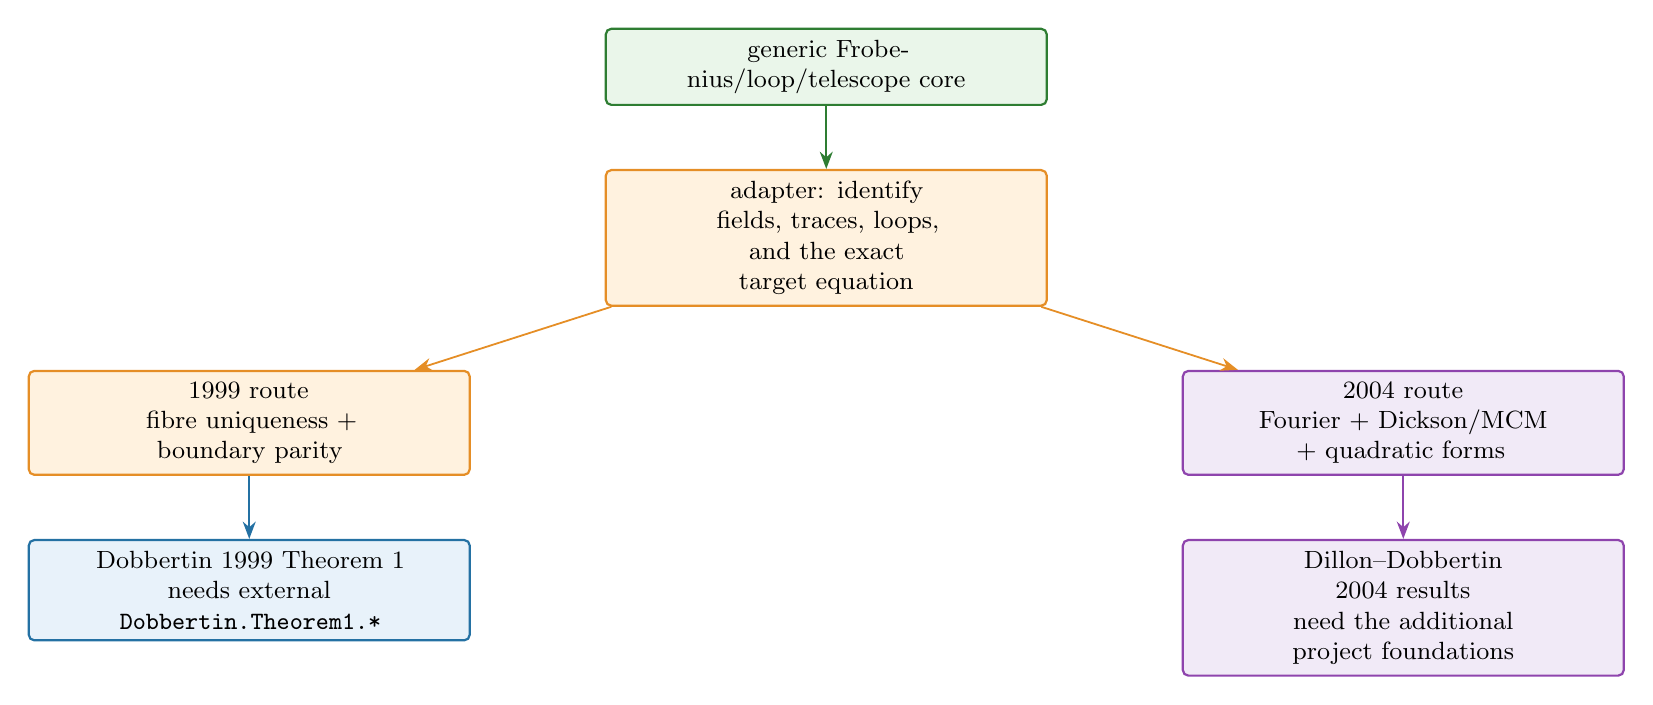
\begin{tikzpicture}[node distance=8mm and 9mm]
\node[sharedbox,minimum width=56mm] (core) at (7.5,.8) {generic Frobenius/loop/telescope core};
\node[partialbox,minimum width=56mm,below=of core] (adapt) {adapter: identify fields, traces, loops,\\and the exact target equation};
\node[partialbox,minimum width=56mm,below left=of adapt,xshift=-8mm] (p99) {1999 route\\fibre uniqueness + boundary parity};
\node[paperbox,minimum width=56mm,below right=of adapt,xshift=8mm] (p04) {2004 route\\Fourier + Dickson/MCM + quadratic forms};
\node[legobox,minimum width=56mm,below=of p99] (th1) {Dobbertin 1999 Theorem 1\\needs external \file{Dobbertin.Theorem1.*}};
\node[paperbox,minimum width=56mm,below=of p04] (tha) {Dillon--Dobbertin 2004 results\\need the additional project foundations};
\draw[arr,shared] (core)--(adapt); \draw[arr,partial] (adapt)--(p99); \draw[arr,partial] (adapt)--(p04);
\draw[arr,legoOnly] (p99)--(th1); \draw[arr,paperonly] (p04)--(tha);
\end{tikzpicture}
\end{center}

\subsection*{Four answers to ``can be built from the same blocks?''}
\begin{enumerate}[label=\arabic*.]
\item \textbf{The generic trace/telescope layer: yes.}  The ZIP deliberately abstracts this layer
      farther than the paper-facing project, including commutative-algebra and categorical versions.
\item \textbf{The 2004 linearized-polynomial subarguments: often, after adapters.}  Definitions and
      exponent conventions must be matched, and the target kernel/fibre theorem still has to be proved.
\item \textbf{The complete 2004 paper: no, not from those blocks alone.}  Its Fourier, difference-set,
      Dickson-torus, quadratic-form, Gauss-sum, and design-theory layers are independent additions.
\item \textbf{The complete ZIP facade: not from the archive alone.}  Its last three modules refer to
      unbundled \file{Dobbertin.Theorem1.*} dependencies.  This does not invalidate the generic core,
      but it prevents treating the ZIP as a standalone complete proof package.
\end{enumerate}

\subsection*{Recommended integration boundary}
Do not merge the two theorem namespaces wholesale.  Extract or import only a small neutral layer:
\[
\boxed{\operatorname{iterSum}}\quad\boxed{\operatorname{Frob}}\quad
\boxed{\operatorname{loop}}\quad\boxed{\text{telescope}}\quad
\boxed{\text{finite-order/fixed-point lemmas}}.
\]
Then prove project-local bridge lemmas to \file{RequestProject.Tr}, partial traces,
\file{MCM_telescope}, and the relevant linearized maps.  This preserves discoverability and avoids
forcing the 2004 library through the ZIP's 1999-specific equations or categorical facades.
\newpage

% ---------------------------------------------------------------------------
\section*{7. File-finder: where to look first}

\begin{tabularx}{\linewidth}{>{\bfseries}p{31mm} X X}
\toprule
Question & First ZIP file(s) & First project / paper location \\
\midrule
Where is the abstract telescope? & \file{DobbertinLego/Endo.lean} & \file{Foundations/LinearizedPoly.lean}; conceptual uses in 2004 \S3--4\\
Where is Frobenius made additive? & \file{Frobenius.lean}; general base in \file{GenBase.lean} & \file{Foundations/TraceLemmas.lean}; used from 2004 \S1 onward\\
Where are trace sums one loop? & \file{Loop.lean}, \file{Assembly.lean} & \file{Basic.lean}, \file{TraceLemmas.lean}; 2004 p.~344 (PDF 3)\\
Where is equation linearization? & \file{Assembly.lean}, \file{AlgebraLayer.lean} & \file{LinearizedPoly.lean}, \file{LopKernelCube.lean}; 2004 \S3 and Appendix A\\
Where are finite fibres counted? & \file{FiberReduction.lean}, \file{FiberUniqueness.lean} & \file{Basic.mult}, \file{CyclicFibre.lean}, \file{Dickson.lean}; Prop.~5 pp.~353--354 (PDF 12--13)\\
Where is additive Fourier theory? & not in the ZIP & \file{AdditiveChar.lean}, \file{Basic.lean}; 2004 pp.~344--345 (PDF 3--4)\\
Where are difference sets? & no dedicated ZIP module & \file{DifferenceSets.lean}; Definition 1/Prop.~2 pp.~345--347 (PDF 4--6)\\
Where is Dickson theory? & not in the ZIP & \file{NormTorus.lean}, \file{DicksonTorus.lean}, \file{Dickson.lean}; 2004 \S3\\
Where is MCM theory? & only generic trace tools & \file{MCM.lean}, \file{MCMDicksonRelation.lean}; Thms.~8--10 pp.~359--360 (PDF 18--19), Thm.~B p.~370 (PDF 29)\\
Where are quadratic forms? & not in the ZIP & \file{QuadFormChar2.lean}, \file{QuadFormClassification.lean}, \file{QuadraticForms.lean}; Appendix A pp.~381--388 (PDF 40--47)\\
Where are cubic Gauss sums? & not in the ZIP & \file{CubicCharacter.lean}, \file{GaussSums.lean}, \file{GaussSumTheory.lean}; Prop.~A.4 pp.~386--387 (PDF 45--46)\\
Where is final assembly? & \file{Theorem1.lean} (1999, with external imports) & \file{MainTheoremA.lean}, \file{HadamardSpectrum.lean}, \file{NoChungYun.lean} (2004)\\
\bottomrule
\end{tabularx}

\vfill
\begin{center}
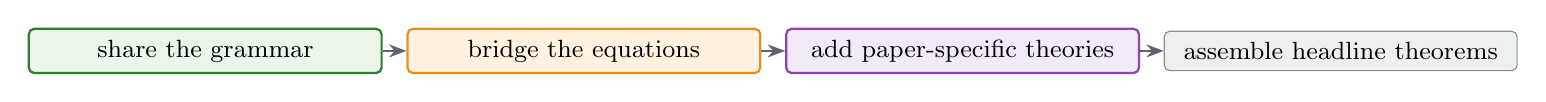
\begin{tikzpicture}[node distance=3mm]
\node[sharedbox,minimum width=35mm] (a) {share the grammar};
\node[partialbox,minimum width=35mm,right=of a] (b) {bridge the equations};
\node[paperbox,minimum width=35mm,right=of b] (c) {add paper-specific theories};
\node[box,fill=ink!8,minimum width=35mm,right=of c] (d) {assemble headline theorems};
\draw[arr] (a)--(b); \draw[arr] (b)--(c); \draw[arr] (c)--(d);
\end{tikzpicture}

\textbf{Bottom line:} one reusable arithmetic chassis, two different mathematical vehicles.
\end{center}

\end{document}
